\documentclass[10pt,twocolumn]{beamer}

\usetheme{Boadilla}
\usecolortheme{crane}
\setbeamertemplate{title page}[default][rounded=true]
\setbeamertemplate{itemize items}[default]
\setbeamertemplate{enumerate items}[default]
\setbeamertemplate{note page}{\pagecolor{cyan!50}\insertnote}
\beamertemplatenavigationsymbolsempty
%\renewcommand{\raggedright}{\leftskip=0pt \rightskip=0pt plus 0cm}

\setbeameroption{hide notes}
%\setbeameroption{show only notes}
%\setbeameroption{show notes on second screen=right}

\usepackage{geometry}
\usepackage{graphicx}
\usepackage{subcaption}
\usepackage{amssymb,amsmath}
\usepackage{bracealign}
\usepackage[none]{hyphenat}
\usepackage[separate-uncertainty=true]{siunitx}

\author{L. Ab'rat}
\title{Investigating Simple Harmonic Motion}
\subtitle{What is a torsional oscillator?}
\date{30 March 1977}
\institute[RHUL]{Royal Holloway, University of London}

\begin{document}

\begin{frame}
	\titlepage
	\setlength{\parskip}{0pt} 
\end{frame}

\begin{frame}
	\frametitle{Resonance}
	\begin{columns}
		\begin{column}{0.37\textwidth}
			From the resonance peak (see Figure), the resonant angular driving frequency, $\omega_D$, is \qty{3.26(2)}{rad~\s^{-1}}.\newline
			
			Using the resonance shift equation (5), we get a value for the natural frequency of \qty{3.28(1)}{rad~\s^{-1}}. This is lower than the predicted value from free oscillations $\left[\qty{3.33(1)}{rad~\s^{-1}}\right]$.
		\end{column}
		\hfill
		\begin{column}{0.57\textwidth}
			\begin{figure}
			\centering
		    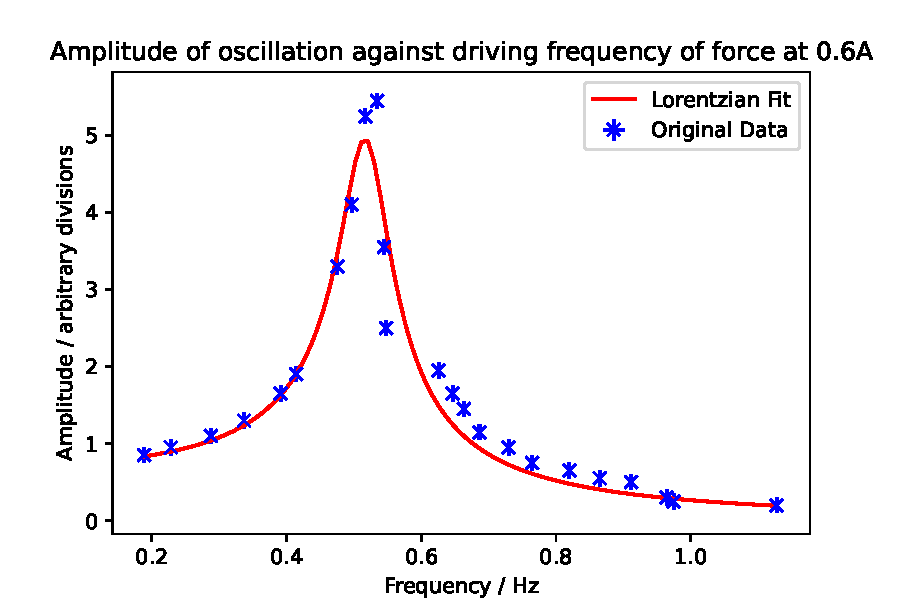
\includegraphics[width=\textwidth]{resonance0.6}
		    \caption{A resonance curve with Lorentzian fit for a damping current of \qty{0.6}{\A}. The peak falls at \qty{0.519(4)}{\Hz}.}
			\end{figure}
		\end{column}
	\end{columns}
\end{frame}

\end{document}